\documentclass[12pt]{kiarticle} % You can learn about my document class "kiarticle" and install it to your device by following the link: https://github.com/Kiarendil/toolkitex
\graphicspath{{pictures/}}
\DeclareGraphicsExtensions{.pdf,.png,.jpg,.eps}
%%%
\pagestyle{fancy}
\fancyhf{}
%\renewcommand{\headrulewidth}{ 0.1mm }
\renewcommand{\footrulewidth}{ .0em }
\fancyfoot[C]{\texttt{\textemdash~\thepage~\textemdash}}
\fancyhead[L]{Дифракция рентгеновских лучей \hfil}
\usepackage{multirow} % Слияние строк в таблице
\newcommand
{\un}[1]
{\ensuremath{\text{#1}}}
\newcommand{\eds}{\ensuremath{ \mathscr{E}}}
\usepackage{tikz}
%%% Работа с таблицами
\usepackage{array,tabularx,tabulary,booktabs} % Дополнительная работа с таблицами
\usepackage{longtable}  % Длинные таблицы
\usepackage{multirow} % Слияние строк в таблице

\usepackage[utf8]{inputenc}
\begin{document}
	
	\begin{titlepage}
	\begin{center}
		\large 	Московский физико-технический институт \\
		(государственный университет) \\
		Факультет инноваций и высоких технологий \\
		\vspace{0.2cm}
		
		\vspace{4.5cm}
		Вопрос по выбору \\ \vspace{0.2cm}
		\large (Общая физика: оптика) \\ \vspace{0.2cm}
		\LARGE \textbf{Дифракция рентгеновских лучей}
	\end{center}
	\vspace{2.3cm} \large
	
	\begin{center}
		Работу выполнила: \\
		\vspace{10mm}		
		
	\end{center}
	
	\begin{center} \vspace{80mm}
		г. Долгопрудный \\
		2020 год
	\end{center}
\end{titlepage}




\section{Рентгеновское излучение}
К рентгеновскому дапазону относят электромагнитное излучение с длиной волны:
\[ 0.1 \ \text{\AA} < \lambda < 100 \ \text{\AA} \]
Разделяют жесткий рентген(<1 \AA), обладающий большой проникающей способностью и мягкий. Жесткий рентген используется, например, в медицинских кабинетах.

Мягкий рентген обладает тем свойством, что он находится в резонансе с электронами внутренних оболочек атомов. Это позволяет использовать его для микроанализа с хорошим пространственным разрешением. Так как максимум излучательной способности плазмы при температурах несколько сотен эВ(такая плазма встречается термоядерных исследованиях и в космических объектах) приходится на мягкий рентгеновских диапазон, то анализ МР-излучения позволяет исследовать космические тела. Так же его используют в литографии и микроскопии.
\section{Формула Лауэ}
Из-за низкой длины волны долгое время не удавалось выявить волновые свойства рентгеновского излучения и пронаблюдать такие явления как дифракция и интерференция. Было предложено использовать кристалл для обнаружения дифракции, поскольку межатомные расстояния по порядку совпадают с длиной волны рентгеновского излучения. Кроме того, атомы в кристаллах расположены регулярно, что позволяло ожидать интерференцию волн, рассеянных группой атомов.

Начнем рассмотрение дифракции рентгеновских лучей с дифракции на прямолинейной цепочке из атомов. Пусть на нее падает излучение под углом $\alpha_0$, тогда разность хода на соседних атомах равна $\Delta = AD - CB = d (\cos \alpha - \cos \alpha_0)$

\begin{wrapfigure}[10]{l}{0.37\linewidth}
    \vspace{-20pt}
	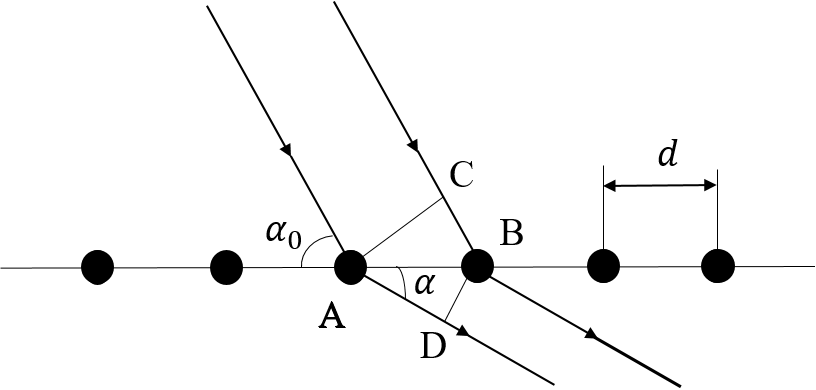
\includegraphics[width=\linewidth]{pic1.png}
	\vspace{-20pt}
	\caption{К выводу формул Лауэ. Дифракция рентгеновского излучения на цепочке атомов}
	\label{ris 1}
\end{wrapfigure}

Условие интерференционного усиления лучей: $\Delta = m \lambda$.

Данное условие наблюдения максимумов можно обобщить на трехмерную периодическую решетку. Пусть на нее падает параллельный пучок рентгеновских лучей, образующий углы $\alpha_0$, $\beta_0$, $\gamma_0$ с координатными осями $X$, $Y$, $Z$. Чтобы волны, рассеянные всеми атомами в направлении прямой, составляющей углы $\alpha$, $\beta$, $\gamma$, с координатными осями, имели максимум по этому направлению, должны выполняться соотношения, называемые условиями Лауэ:
\begin{equation*}
    d_1 ( \cos \alpha - \cos \alpha_0) = m_1 \lambda,
\end{equation*}
\begin{equation*}
    d_2 ( \cos \beta - \cos \beta_0) = m_2 \lambda,
\end{equation*}
\begin{equation*}
    d_3 ( \cos \gamma - \cos \gamma_0) = m_3 \lambda.
\end{equation*}

Каждое из этих условий необходимо, чтобы происходило интерференционное усиление волн, рассеянных под соответствующими углами к осям. Кроме того, эти условия являются достаточными для наблюдения максимума в конкретном направлении рассеяния всеми атомами. 

\section{Лауэграмма}
\begin{wrapfigure}[15]{r}{0.25\linewidth}
    \centering
    \vspace{-30pt}
	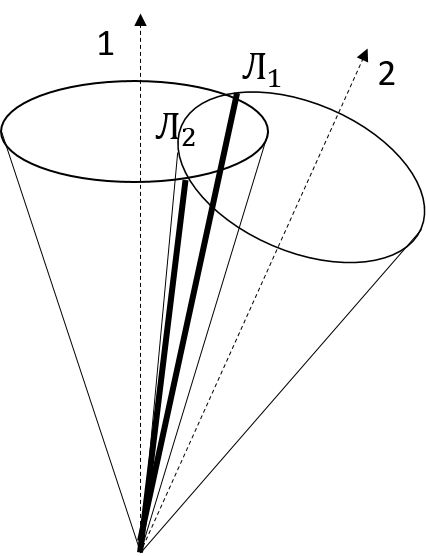
\includegraphics[width=\linewidth]{pic4.png}
	\caption{К Лауэграмме. Линии Л1 и Л2 - линии пересечения конусов максимумов дифракции на осях 1 и 2}
	\label{ris 3}
\end{wrapfigure}
Лауэграмма - дифракционная картина, образованная рентгеновскими лучами, рассеянными кристаллом.
Условия Лауэ задают три конуса, образующих углы $\alpha$, $\beta$, $\gamma$ с осями $X, Y, Z$ соответственно. Интенсивность будет максимальна, когда дифрагированный пучок лежит на поверхности всех трех конусов. Но три конуса в общем случае не пересекаются по общей прямой. Поэтому для получения лауэграмм от кристаллов используется рентгеновское излучение с широким сплошным спектром, так как в таком спектре могут присутствовать такие длины волн, для которых выполняются условия Лауэ. В упрощенном предположении, для равных периодов по всем направлениям разрешим условия Лауэ относительно длины волны:
\[ \lambda = -2 \frac{m_1 \cos \alpha_0 + m_2 \cos \beta_0 + m_3 \cos \gamma_0}{m_1^2 + m_2^2 + m_3^2} d. \]

\section{Формула Брэгга-Вульфа}
Дифракцию рентгеновских лучей на кристалле можно трактовать еще одним способом. Рассмотрим схему, называемую брэгговским отражением, которая так же позволяет рассчитать дифракцию. Введем атомные плоскости - плоскости, содержащие большое число атомов и расстояние d между ними. Тогда при падении параллельного пучка произойдет его отражение от разных плоскостей, и в результате мы получим интерференционную картину таких отраженных волн. 
\begin{figure}[H]
	\begin{center}
		\begin{minipage}[h]{0.4\linewidth}
			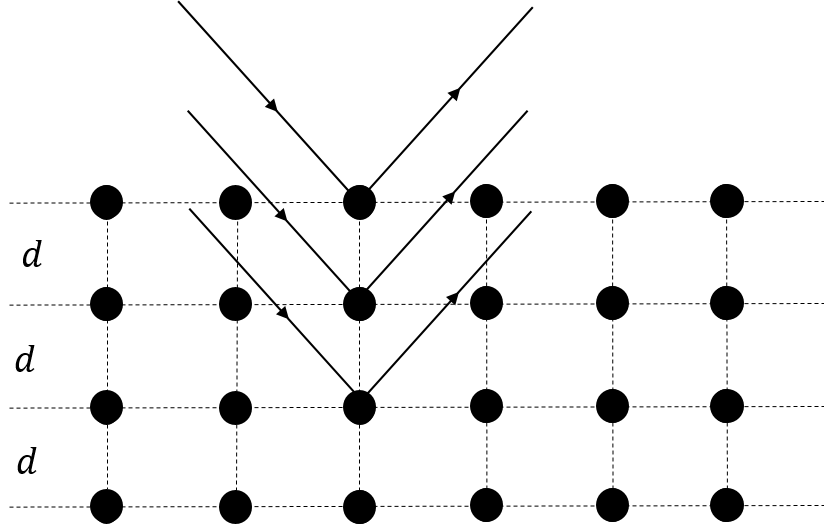
\includegraphics[width=1\linewidth]{pic2.png}
			\caption{К выводу формулы Брегга-Вульфа} 
			
		\end{minipage}
		\hfill
		\begin{minipage}[h]{0.4\linewidth}
			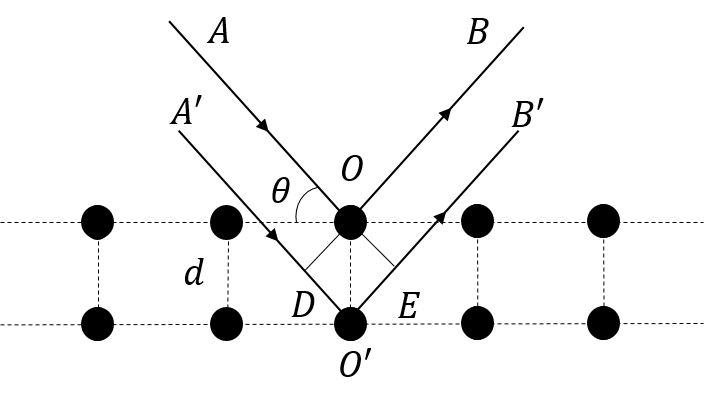
\includegraphics[width=1\linewidth]{pic3.png}
			\caption{Дифракция рентгеновского излучения на атомах}
			
		\end{minipage}
	\end{center}
\end{figure}
Разность хода между лучами, отраженными от соседних плоскостей $\Delta = 2 d \sin \theta$. Для интерференционного усиления должно выполняться условие, называемое условием Брэгга-Вульфа: 
\[ 2 d \sin \theta = m \lambda\]

Можно показать, что условия Брэгга-Вульфа и Лауэ эквивалентны, а значит все направления на максимум, даваемые одним условием, будут следовать и из второго. 

\section{Применение. Рентгеновский спектрограф}
Открытие дифракции рентгеновских лучей подтвердило их электромагнитную природу, а также доказало периодическую структуру кристаллов. Это положило начало таким направлениям как рентгеноструктурный анализ и рентгеновская спектроскопия. Рентгеновская спектроскопия использует естественные кристаллы известной кристаллической структуры для анализа рентгеновского излучения и измерения длин волн. Рентгеноструктурный анализ, наоборот, использует рентгеновское излучение известной длины волны для выяснения кристаллической структуры кристаллов и измерения параметров этой структуры.

\begin{figure}[H]
	\begin{center}
		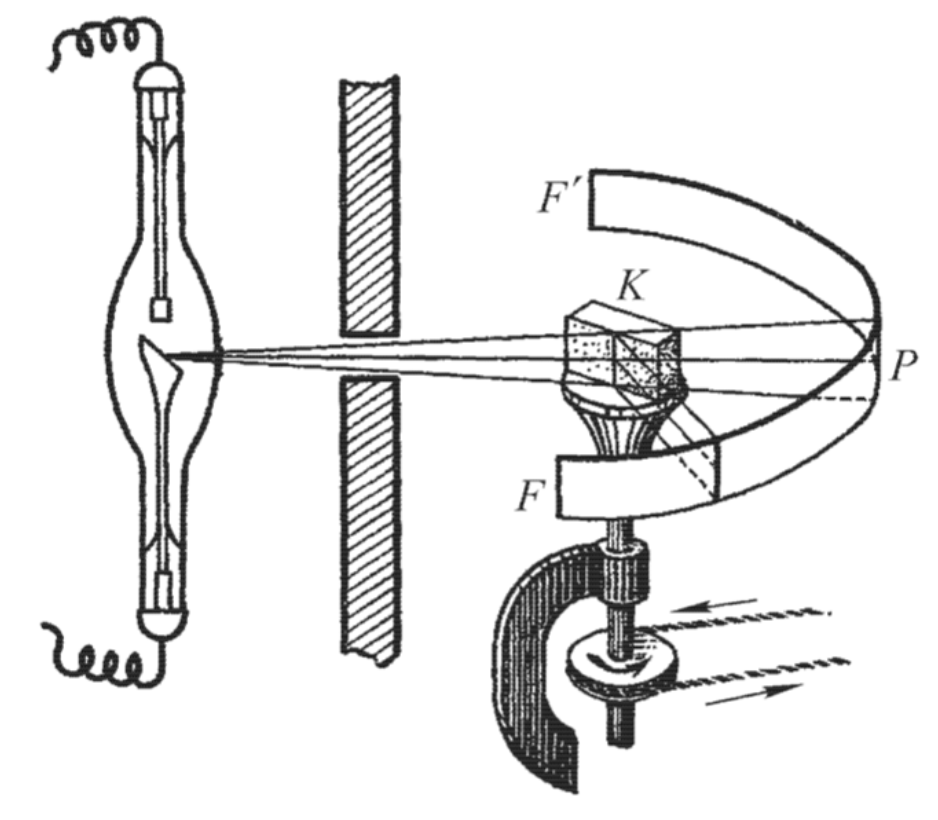
\includegraphics[width=0.6\linewidth]{pic5.png}
		\caption{Схема рентгеновского спектрографа} 
	\end{center}
\end{figure}
\vspace{-30pt}
Рассмотрим рентгеновский спектрограф с вращающимся кристаллом. Рентгеновский пугеновский пучок после диафрагмирования на щелях направляется на монокристалл К известной кристаллической структуры.
Кристалл может вращаться вокруг оси, перпендикулярной к падающему лучу. Дифрагированный пучок попадает на фотопластинку FF'. При произвольном положении кристалла условие Брэгга-Вульфа может быть невыполнено, если пучок монохроматичен. Однако при повороте кристалл может занять такое положение, при котором это условие выполняется. Тогда возникнет отраженный максимум, регистрируемый фотопластинкой. Найдя такое положение, можно определить угол скольжения, а по нему длину волны.



\section{Метод Дебая-Шерера-Хелла}
Метод применяется в рентгеноструктурном анализе для исследования кристаллической структуры материалов в порошкообразном состоянии. Поликристалл состоит из множества мельчайших кристалликов, беспорядочно ориентированных во всевозможных направлениях. В отличии от рентгеновского спектрографа образец неподвижен. На него направляется монохроматический рентгеновский луч с известной длиной волны $\lambda$. Дифракционная картина, называемая дебаеграммой, фотографируется.
Среди множества беспорядочно ориентированных кристалликов найдется большое количество с такими ориентациями, что при заданной длине волны будет выполнено условие Брэгга-Вульфа. Лучи, испытавшие брэгговские отражения от таких кристалликов, образуют поверхность конуса, ось которого направлена вдоль падающего луча, а угол раствора определяется межплоскостным расстоянием $d$. Так как эти расстояния образуют дискретный набор, то за образцом возникнет дискретное семейство конусов с общими вершиной и осью.

Если бы фотопластинка была установлена перпендикулярно к этой общей оси, то дебаеграмма состояла бы из концентрических кругов. Измерив радиусы этих кругов, можно определить возможные значения угла $\theta$, а затем по формуле Брэгга-Вульфа вычислить соответствующие межплоскостные расстояния и воспользоваться этими данными для воспроизведения кристаллической структуры образца.
Чтобы получить действительно все межплоскостные расстояния, фотопластинке придают форму полоски, опоясывающей по окружности исследуемый образец.

\begin{figure}[H]
	\begin{center}
		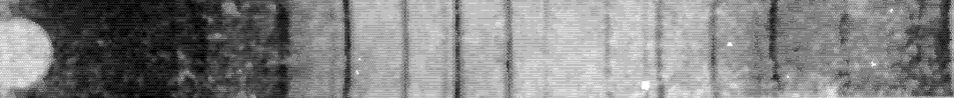
\includegraphics[width=0.8\linewidth]{pic6.png}
		\caption{Дебаеграмма, полученная на кристаллическом порошке $\rm NaCl$} 
	\end{center}
\end{figure}
\vspace{-30pt}

\end{document}
